\chapter{Conclusion}
The main idea behind developing this application was to create a software environment similar to what I might encounter after finishing my degree, such as using agile technologies to build a full stack social media application, testing the application, and creating behavior driven environment so that anyone could understand how the application should work. The application is then deployed online, and finally, a highly appealing front end look and pleasing UI were created for the application.

\section{Aims}
The purpose of creating the application, what I expected to achieve during the development of the website, and did I met my personal aims.
\begin{itemize}
    \item To build a highly pleasing front-end website, which will have a great appearance to please all who visit the application.
    \item To create multiple test scenarios, and have such scenarios fully automated using cypress.
    \item To improve my website design skills using React and JavaScript.
    \item To further my ability using automated testing.
\end{itemize}

\subsection{Aim One}
I felt I had created a stylish dynamic front end application that promotes ease of use and isn't overly cluttered, with what I consider to be a simple but elegant feel to the CSS and HTML placements of the cards, navigation bar, and form, combined with a small amount of color in the logo and background, alluding to the application not being overly cluttered.

\subsection{Aim Two}
This is my first time using behavior driven development, and I believe I designed and created test scenarios that promote ease of reading and use. I believe this is how I will develop applications from now on, writing gherkin scenarios, and incorporating such features with the development of the application, allowing testing and development to occur concurrently. When combined with cypress, it helps me achieve my fourth aim.

\subsection{Aim Three}
Throughout the course of creating this application, I have gained a much greater understanding of using JavaScript and integrating functions in JS to be used between the front end and the back end. Additionally, I am much more comfortable using React as a front end architecture, especially using this technology in conjuncture with JSX, which provides the programmer ample more control over the UI. 

\subsection{Aim Four}
Using automated testing is a real eye opener, such testing is superior, in terms of tracking metrics in which I can see what parts of the application are working as expected, and to view which sections of the application aren't working as expected. It was a great skill to pick up throughout the building of this application and I hope to carry it onward into a workplace environment using behaviour driven development.

\newpage
\section{Jira Roadmap}
A comparison of my agile roadmap, how the project occurred during the course of the year versus how I thought the project would go in my Gantt chart \ref{image:GanttChart}.
\begin{figure}[h!]
    \centering
    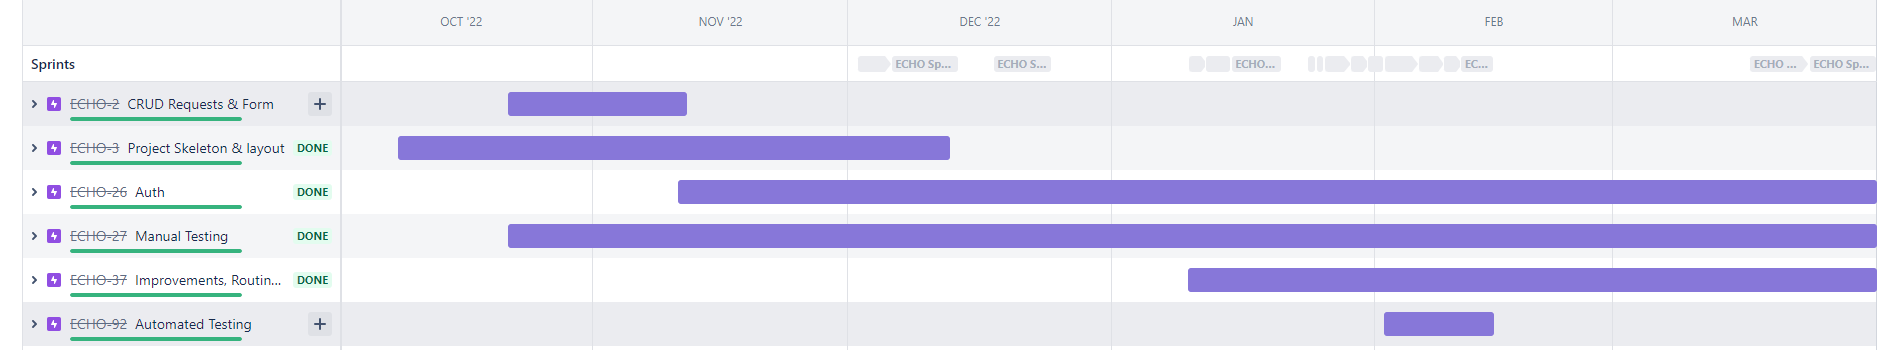
\includegraphics[width=0.8\textwidth]{images/AgileBoard.png}
    \caption{Agile Board}
    \label{image:AgileBoard}
\end{figure}


\section{Other Learning's}
Supplementary education I received during the course of creating the application.

\subsection{Using JSON}
I had already previously used JSON, however during the time spent on this project I used JSON Web Token(JWT) in order create a unique signature for a signed in user thereby allowing authorization to function properly.

\subsection{Creating a dynamic single page application}
Creating an SPA, which is a popular industry method for building applications that are quick and efficient.

\subsection{Using REST}
Learning more about creating a RESTful application, this would be used in conjuncture with JSON from above, and HTTP methods for declaring how the application should present the data.

\subsection{Model View Controller}
After studying the theory of MVC during my tenure at ATU, I was proud to be able to put it into practise in the back end of my project, it gave the back end substantial organisation when an addition to the application was made.

\section{Succeeding in Objectives?}
How well objectives were met was discussed in chapter \ref{chap:Eval}. However, the findings from the evaluation chapter are as follows, the system works like a dynamic single page application, authorization, search, comments and creating posts were all achieved, however creating a chat environment was not accomplished, all of the above was validated through Cypress automated test suite, and manual testing, using behaviour driven test scenarios. Limitations of the application can be seen here \ref{sec:Limit}, below is the possible future of the application.

\section{The Applications Future}
In the future I hope to add features such as having a forgotten password feature, machine learning to predict what the user wishes to search, having a real time chat in the post details section of the application, and putting the cypress tests into a pipeline like for instance Microsoft azure.

\section{Credit}
I would like to take this moment to thank my supervisor Martin Hynes who was a tremendous help throughout the project.
